\documentclass[11pt,a4paper]{extarticle}
\usepackage[utf8]{inputenc}
\usepackage[spanish]{babel}
\usepackage{amsmath}
\usepackage{amsfonts}
\usepackage{amssymb}
\usepackage{graphicx}
\usepackage[left=1.2cm,right=1.2cm,top=2cm,bottom=2cm]{geometry}
\date{\small{\today}}
\usepackage{fancyhdr}
\usepackage{afterpage}
\usepackage{titlesec}
\usepackage{float}
\usepackage{gensymb}
\usepackage{xfrac}
\usepackage{tabularx}
\usepackage{multicol}
\usepackage[font=small]{caption}
\usepackage{scrextend}
\usepackage[toc,page]{appendix}

\renewcommand\appendixpagename{Apéndices}
\renewcommand\appendixname{Apéndice}

\titleformat{\section}{\Large\bfseries}{}{0em}{}[]
\titleformat{\subsection}{\large\bfseries}{}{0em}{}[]
\titleformat{\subsubsection}{\bfseries}{}{0em}{}[]
\titleformat{\chapter}{\large\bfseries}{}{0em}{}[]


\setlength\parindent{0pt}


\begin{document}
\title{Implementación de Amplificador Lock In Dígital}
	\LARGE{\textsc{Laboratorio II}}\\
	\Large{Implementación de Amplificador Lock-In Dígital}\\
\begin{large}
\small\textsc{Horst, Raúl Tomás}\\
\small\textsc{Roqueta, Matías Daniel}\\
\small{Centro Atómico Bariloche y Instituto Balseiro, Comisión Nacional de Energía Atómica}\\
\end{large}
\setcounter{page}{1}

\lhead{Laboratorio II}%Materia
\rhead{Implementación de Amplificador Lock-In Dígital}%Título 
\chead{}

\lfoot{R. Horst, M. Roqueta}
\cfoot{Instituto Balseiro} 
\rfoot{\thepage} 
\renewcommand{\headrulewidth}{0.4pt} 
\renewcommand{\footrulewidth}{0.4pt} 
\pagestyle{fancy}

\hrule
\begin{multicols}{2}
\normalsize
\section{Resumen}

\section{Introducción}

Un amplificador lock in es un dispositvo electrónico capaz de extraer la fase y amplitud de una señal de banda angosta medida en un ambiente ruidoso.\\

El funcionamiento del lock in equiere información de la dependencia temporal de la señal de interés, que es aportada por una señal de referencia. Según la implementación, la señal de referencia puede ser inyectada al lock in de una fuente externa o generada internamente.\\ 

El lock in recupera la señal de interés multiplicando a esta por la referencia en fase y cuadratura, y aplicando un filtro pasa bajo al producto de señales. Este proceso es llamado \textit{demodulación coherente}.\\

\begin{figure}[H]
	\centering
	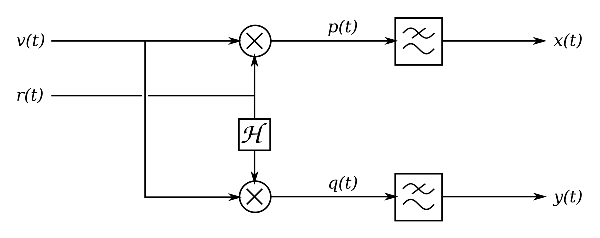
\includegraphics[width=\linewidth]{Images/lockin_gral.eps}
	\caption{Una señal de entrada $v(t)$ es inyectada al lock in. Posterior a la demodulación coherente, se extrae la señal de interés $z(t)=x(t)+jy(t)$}
	\label{fig:lockin}
\end{figure}

La figura \ref{fig:lockin} presenta un circuito lock in típico. El bloque transformada de Hilbert para una referencia senoidal corresponde a un desfasaje de 90°. La señal de salida se obtiene en forma de parte real e imaginaria, pero típicamente se expresa en forma amplitud y fase

\begin{equation*}
	z(t) = x(t) + j y(t) = R(t) e ^{j\Phi(t)}
\end{equation*}\\[-1em]

Donde la amplitud y fase se obtienen de las ecuaciones

\begin{equation*}
	R(t) = \sqrt{x^2(t)+y^2(t)} \qquad \qquad \Phi(t) = \arctan\frac{y(t)}{x(t)}
\end{equation*}\\


Para comprender el comportamiento esperando del demodulador coherente resulta útil visualizar las señales involucradas en el dominio de la frecuencia, análisis que se realiza en la figura \ref{fig:sigs_fourier}.

\begin{figure}[H]
	\centering
	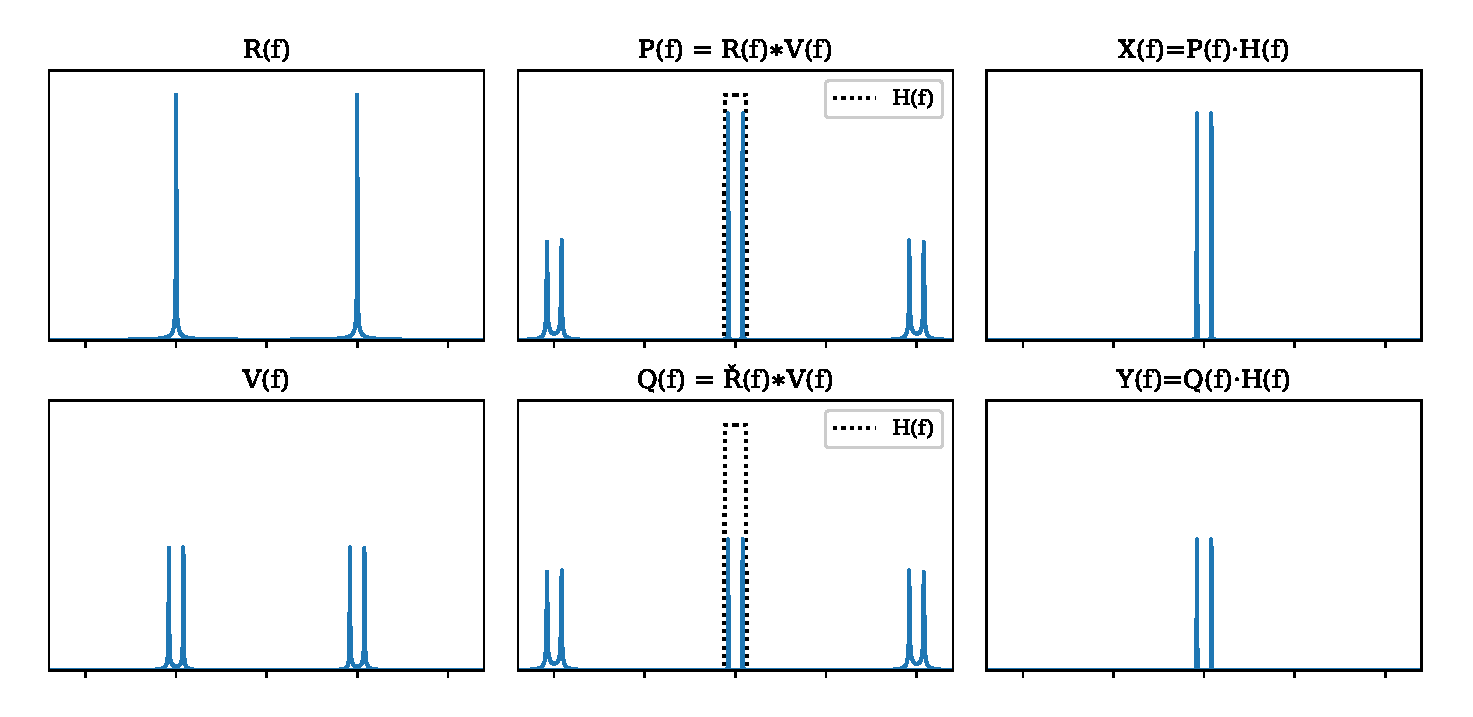
\includegraphics[width=\linewidth]{Images/sigs_fourier.eps}
	\caption{Realización en ausencia de ruido de las señales presentes en la figura \ref{fig:lockin} representadas en el dominio de la frecuencia, incluida la respuesta en frecuencia del filtro.}
	\label{fig:sigs_fourier}
\end{figure}

La salida $z(t)$ del demodulador coherente se puede interpretar como la entrada $v(t)$ transportada a banda base. Por este motivo la frecuencia de corte del filtro pasa bajos se debe elegir tal que acepte el ancho de banda de la señal a medir.

\section{Implementación}

La aplicación del amplificador lock in correspondiente a la práctica realizada es de medición de impedancias. Esto se realiza midiendo la transferencia de un circuito divisor de tensión con una impedancia incógnita.

\begin{figure}[H]
	\centering
	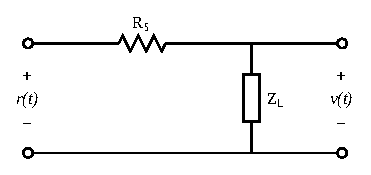
\includegraphics[width=0.75\linewidth]{Images/transferencia.eps}
	\caption{Circuito a medir, $R_S$ es una resistencia de valor conocido, y $Z_L$ una impedancia supuesta incógnita.}
	\label{fig:transferencia}
\end{figure}

En estas condiciones, se mide 
\begin{equation}
	H = \frac{v(t)}{r(t)} = \frac{Z}{R + Z} \quad \longrightarrow \quad Z =  \frac{HR}{1-H}	
\end{equation}

La relación $v(t) = H r(t)$ con $H \in \mathbb C$ implica que el ancho de banda de la señal a medir puede considerarse arbitrariamente chico.\\

El filtro elegido fue un FIR digital por su simplicidad de implemntación. Aplicar el filtro de orden N se reduce a un único producto interno vectorial

\begin{equation}\label{eq:fir}
	y_i = \sum_{j=0}^N h_jx_{i-j}= 
	\begin{bmatrix}
		x_i & \cdots & x_{i-N}
	\end{bmatrix}
	\begin{bmatrix}
		h_0 \\ \vdots \\ h_N	
	\end{bmatrix}
\end{equation}\\[-1em]

El filtro FIR es generado con la función \texttt{firwin} perteneciente a \texttt{scipy.signal} que garantiza fase constante, lo que permite fácilmente conocer su retardo de grupo a frecuencia de muestreo $f_s$

\begin{equation}\label{eq:tau}
	\tau = \frac{N-1}{2f_s}
\end{equation}\\[-1em]

Ya que lo que interesa medir en nuestro circuito es transferencia, resulta útil normalizar los valores a fin de independizar la medición de la tensión de alimentación del circuito y medir la transferencia diréctamente. El lock in implementado corresponde a la figura \ref{fig:nuestro_lockin}

\begin{figure}[H]
	\centering
	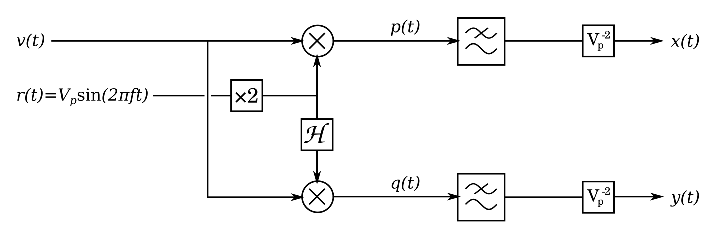
\includegraphics[width=\linewidth]{Images/nuestro_lockin.eps}
	\caption{Lock In implmentado para medición de impedancias. El módulo $\times 2$ aplicado a la referencia contrarresta un efecto de la demodulación visto en la figura \ref{fig:sigs_fourier} donde la mitad de la amplitud de la señal de interés es transportada a alta frecuencia y filtrada.}
	\label{fig:nuestro_lockin}
\end{figure}

\section{Método Experimental}
En primer lugar se midió la frecuencia máxima de 
sampleo que permitía el dispositivo de medición.\\

Luego se ensambló el circuito de la figura 
\ref{fig:transferencia}, en donde $ZL$ era de carácter
 puramente resistivo, y se pudo obtener 
el valor de la resistencia de carga $RL = ZL$ para 
comprobar el funcionamiento del lock in en el caso 
de impedancias reales.\\ 

Se utilizaron dos generadores de señal RIGOL DG4102 
para poder generar la señal de referencia y el ruido.
Para sumar éstas dos señales se tuvo que "flotar"[1] la 
tierra de uno de los generadores dado que éstos no poseen 
tierra propia, sino que utilizan la de la red eléctrica.\\

Para la realización del lock in se implementó un 
script en python como se puede ver en el apéndice.
En el código se importó la librería del dispositivo 
de medición, el 
conversor analógico dígital USB-1408FS de la línea 
MEASUREMENT COMPUTING, para poder 
calibrarlo y realizar las mediciones.\\

Se implementaron 
las etapas de la figura \ref{fig:nuestro_lockin},
 en donde se optó por utilizar filtros FIR dada 
 su versatilidad y sencillez.\\

El programa toma la señal $v(t)$
y la normaliza utilizando su máximo valor de amplitud,
 siendo ésta la tensión de referencia. Además se mide 
 la señal $r(t)$ y se le aumenta la amplitud en un factor
 de 2 por el desarrollo que se necesita [Apéndice].
Se genera la señal $p(t)$ mediante la multiplicación de 
las dos señales tomadas.
Luego se genera la señal $q(t)$ desfasando 90◦
la señal 
mediante la transformada de Hilbert.
Por último se aplican filtros pasa bajos,
 obteniendo respectivamente las salidas $x(t)$ e $y(t)$,
  necesarias para obtener los
valores de amplitud y fase de la señal $v(t)$.


\section{Resultados}

Falta analizar que puntos usar de las gráficas y reportar
el valor RL = ... +/- ..., CL = ... +/- ...\\

Se determinó que la frecuencia máxima de muestreo es 
de aproximadamente 
500Hz, con una frecuencia máxima medible de 250Hz, 
según el teorema de muestreo de Nyquist[2].\\

Se midió el valor de $RL$ en función 
de la relación señal a ruido en la entrada para tres 
filtros FIR de distinto orden.
Se puede apreciar que el filto óptimo es el de mayor 
orden, dado que se utilizan mayor cantidad de 
mediciones para generar las señales medidas.

\begin{figure}[H]
	\centering
	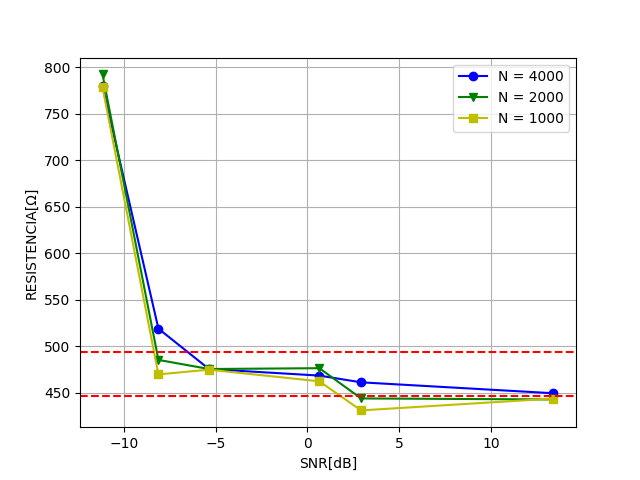
\includegraphics[width=\linewidth]{Images/RvsSNR(segunda).png}
	\caption{RvsSNR}
	\label{fig:RvsSNR}
\end{figure}

Para comprobar que el límite de funcionamiento 
del lock in no está limitado por el orden del 
filtro elegido sino por la SNR a la entrada
se realizaron distintas mediciones 
sobre el valor $RL$(dada la simpleza del circuito) 
para un valor de SNR a la entrada de -22.5dB para 
distintos filtros como se explaya en la figura 
\ref{fig:RORDEN}. Se aprecia un valor mas acercado 
al tabulado cuando se aumenta el orden del filtro, sin 
embargo está lejos de entrar en la cota del error 
tabulado, y ésto asegura que el limitante en éste 
lock in es el ruido a la entrada.\\

Cabe aclarar que los valores de resistencia que estamos
 midiendo están dos ordenes de magnitud por de 
 bajo de la impedancias de entrada del dac, y al estar en 
una conexión en paralelo predomina el valor de la resistencia 
que deseamos obtener.\\

\begin{figure}[H]
	\centering
	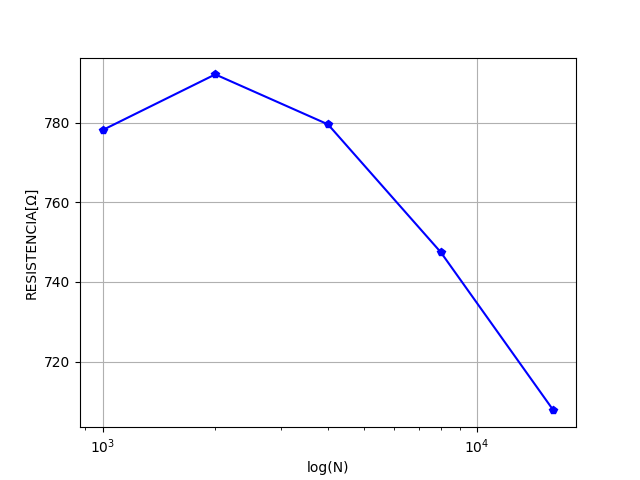
\includegraphics[width=\linewidth]{Images/RORDEN.png}
	\caption{RORDEN}
	\label{fig:RORDEN}
\end{figure}

Por último se armó el circutio de la figura 
\ref{fig:CvsSNR} .Con ésto 
se midió el valor de la capacidad $CL$ para poder 
comprobar el funcionamiento del lock in en 
impedancias complejas.\\ 

\begin{figure}[H]
	\centering
	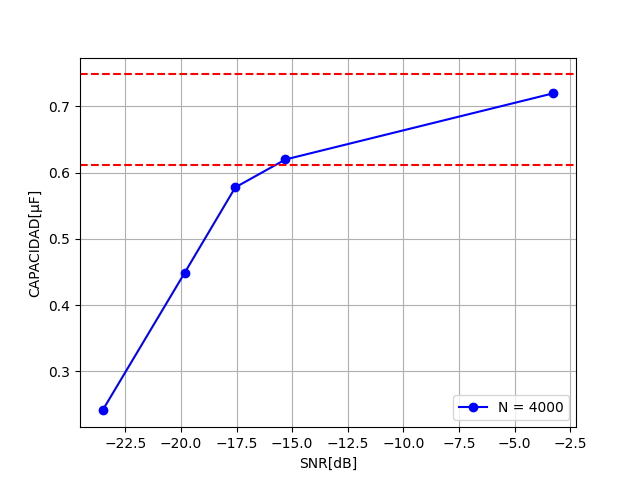
\includegraphics[width=\linewidth]{Images/CvsSNR(segunda).png}
	\caption{RvsSNR}
	\label{fig:CvsSNR}
\end{figure}


\section{Discusión}
Discusión o trabajo a futuro:\\
-Frecuencia de muestreo ¿usar otro dac?\\
-Orden del filtro\\
-Pq tuvimos que flotar\\
-Hacer más mediciones en el capacitor entre -5dB y -15db, 
porque en la resistencia llega hasta -12dB como mínimo.
Con respecto a ésto, ¿descartamos 4 puntos en el gráfica de 
la capacitancia?, nos quedaría sólo 1...

\section{Conclusiones}

Si bien los amplificadores lock in comerciales resuelven 
mediciones con SNR de 1:1000, se encuentra satisfactorio 
el rendimiento del lock in digital desarrollado, con 
una implementación relativamente sencilla.\\

Se concluye que la mínima SNR de entrada para el 
correcto funcionamiento del lock in implementado es de 
aproximadamente unos "-6dB por ejemplo".(VER BIEN QUE 
CRITERIO UTILIZAR PARA DAR EL VALOR, y si 
conviene en dB o en 1:10 por ejemplo)

\section{Referencias}

\bibliography{Antenas}
\bibliographystyle{ieeetr}

\end{multicols}
\newpage
\begin{appendices}
\vspace{-1em}
\hrule
\vspace{1em}
\normalsize
\section{Apéndice 1 - apéndice}
\end{appendices}

\end{document}